\documentclass[a4paper, 10pt, conference]{ieeeconf}
\IEEEoverridecommandlockouts
% The preceding line is only needed to identify funding in the first footnote. If that is unneeded, please comment it out.
\overrideIEEEmargins                                      % Needed to meet printer requirements.

\usepackage{cite}
\usepackage{url}
\usepackage{hyperref}
\usepackage{amsmath,amssymb,amsfonts}
\usepackage{algorithm}
\usepackage{algorithmic}
\usepackage{graphicx}
\usepackage{subcaption} 
\usepackage{textcomp}
\usepackage{xcolor}
\def\BibTeX{{\rm B\kern-.05em{\sc i\kern-.025em b}\kern-.08em
    T\kern-.1667em\lower.7ex\hbox{E}\kern-.125emX}}
\newcommand{\fk}[1]{\textcolor{red}{[FK:#1]}}
\title{\textbf{Learning and generalizing tasks on humanoid robots with an automatic multisensory segmentation method}
}

\author{Victor Barberteguy$^{1,2}$ and Fumio Kanehiro$^{2}$
\thanks{$^{1}$Ecole Polytechnique, Palaiseau, France}
\thanks{$^{2}$CNRS-AIST JRL (Joint Robotics Laboratory), IRL, National Institute of Advanced Industrial Science and Technology (AIST), Tsukuba, Japan}
}

\begin{document}

\maketitle
\thispagestyle{empty}
\pagestyle{empty}

\begin{abstract}
We provide a complete framework for learning and reproducing tasks from human demonstrations. This framework adapts recent developments in automatic, unsupervised segmentation of time-series to humanoid robotics by preprocessing the data obtained from a broad range of the robot's sensors, to then repropduce the learned task in similar environments.

In more detail,  we reproduce and extend the acquired multi-step task using Dynamic Movement Primitives in simulation for the JVRC1 Robot, and further validate it the segmentation process in real world with the HRP-4C Robot, thus showcasing the possibility to create an extensive library of reusable skills for complex humanoids with our approach.
\end{abstract}

% \begin{IEEEkeywords}
% learning from demonstration, generalization, teleoperation, probabilistic inference, feature selection, dynamic movement primitives, sensory skill integration
% \end{IEEEkeywords}

\section{Introduction}
\subsection{Learning from Demonstration}

Demonstrations provide an intuitive way for non-professional users to specify tasks to the robot\cite{schaal_is_1999}. Most of robot's controllers to date, albeit successful to achieve complex tasks, often require theoretical knowledge and is time-consuming. To address these issues, research about robot learning from demonstration (LfD) has become increasingly important over the past two decades with the surge of Machine Learning (ML) algorithms\cite{argall_survey_2009,ravichandar_recent_2020}. In this framework, users can demonstrate a task that is then learned and generalized by the robot. Generalization is defined as the capacity to perform a learned task in a similar environment as the one of the demonstration, but under different initial or goal poses. 
%LfD has been widely used and proved successful on robotic arms or in simulation\cite{pastor_learning_2009}, but are more seldom used on real humanoid robots\cite{calinon_learning_2007} due to their high number of degrees of freedom (DoF) and unlinear behavior. A core idea of this work is to capitalize on the physiologic similarities between us, humans, and humanoids robots to come up with an intuitive LfD technique. Consequently, this article showcases a method specific to humanoid robots.


\begin{figure}[t]
  \centering
  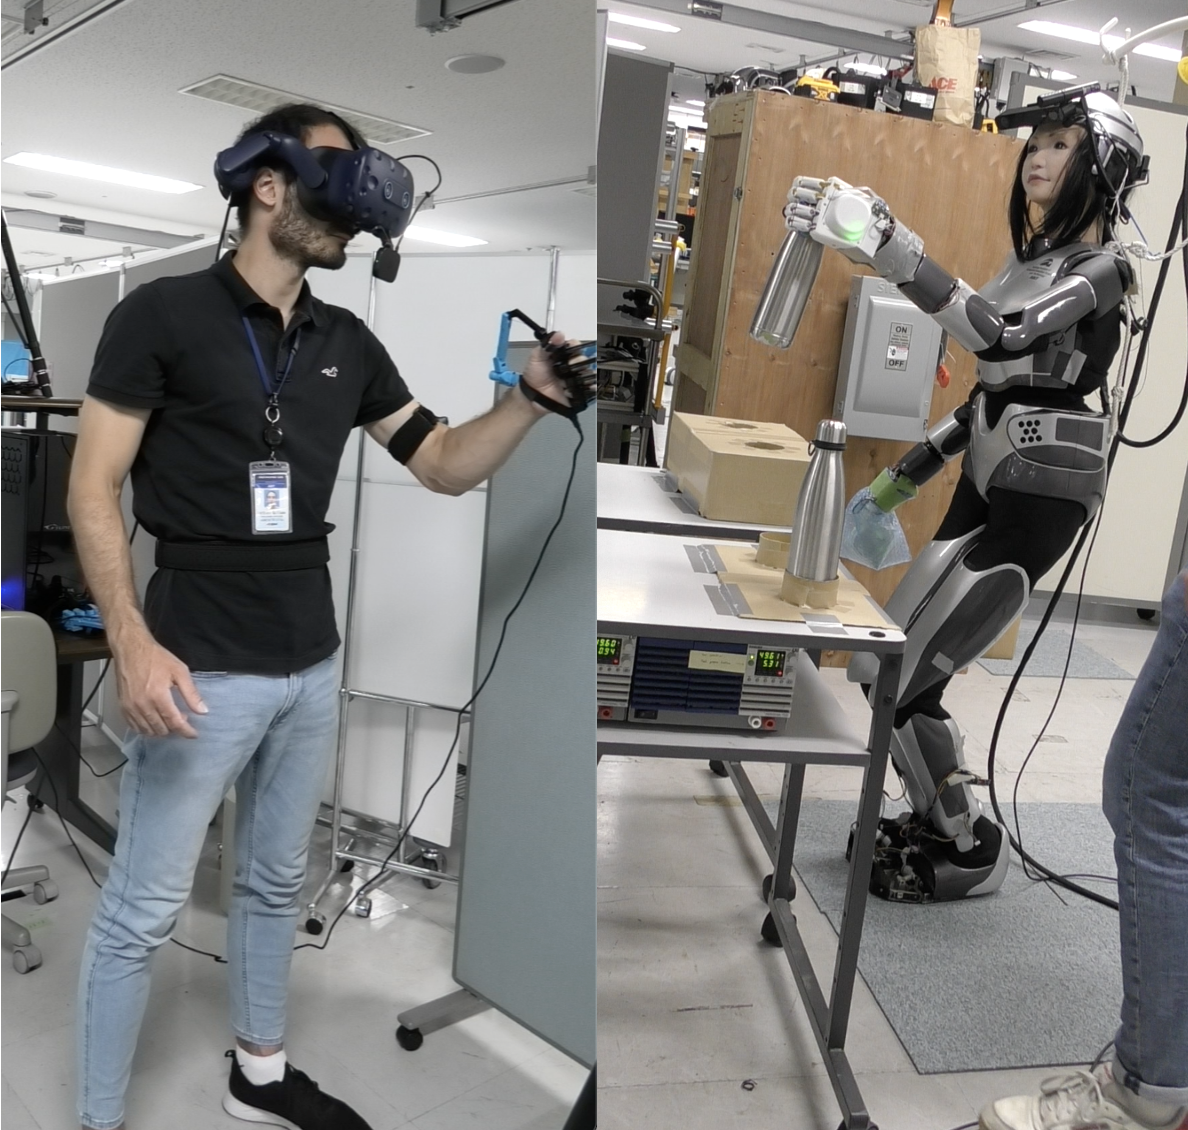
\includegraphics[width=0.45\textwidth]{img/Setup.png}
  \caption{Picture of the experimental setup. On the right, the demonstrator wearing the teleoperation device. On the left, the HRP-4C robot that is teleoperated.}
  \label{fig:setup}
\end{figure}


Several techniques are found in the literature to provide demonstrations to the robot. This can be done through simulation\cite{sammut_learning_1992}, kinesthesic teaching\cite{wu_prim-lafd:_2022}, motion capture\cite{ramirez-amaro_understanding_2015} or with teleoperation devices. 
%These teleoperations devices appear under various shapes, from joysticks \cite{ando_master-slave_2020} to exoskeletons where the user remotely controls the robot \cite{fang_skill_2019}. 

In all the above cited works, some prefer 1-shot imitation learning, where the demonstration can be a seed for an initial policy that is then derived and learned through Reinforcement Learning (RL)\cite{vecerik_practical_2019,stulp_reinforcement_2012}, Inverse RL\cite{rouot_inverse_2017} or Hierarchical RL\cite{zhao_variational_2023} that can possibly be corrected with online coaching\cite{advice_operator}. 
%Another recent approach is to create more demonstrations with the initial one, thus enriching the dataset thanks to meta-learning processes \cite{yu_one-shot_2018}. 
On the contrary, other methods rely on a set of demonstrations to perform probabilistic inference based on Hidden Markov Models\cite{rana_towards_2017}, Neural Networks\cite{zhang_deep_2018} or using Granger Causality\cite{chuck2023grangercausal}. The former often derives only one policy that is locally optima, and thus the learning process is repeated for each task, whereas the latter methods prefer to decompose the task in elementary \textit{skills} with segmentation methods, thus enhancing the reusability of the stored skills. Our framework is of the latter category, that is further detailed in \ref{Approach}. Whatever the method used, once the task learned, the great majority of the references cited above use Dynamic Movement Primitives (DMP)\cite{ijspeert_movement_2002,ijspeert_dynamical_2013} that provides a suitable framework to reproduce trajectories and smoothly adapt to new conditions. 
%This research aims to build a framework that enables humanoid robots to learn, reproduce and generalize manipulation tasks using such DMPs as well as time-series segmentation techniques.

\subsection{Segmentation of the tasks} \label{Approach}

Splitting a complex task such as grasping an object or pouring water has the advantage of making the result more generalizable. Indeed, every part of the trajectory (every \textit{skill}) has its own level of generalizability thanks to DMP, thus resulting in an intra-task generalization, better than a single end-to-end DMP. Nonetheless, a complex task is almost all the time demonstrated without specifying the number of segments: the demonstrator naturally achieves the task. Consequently, one challenge of this approach is to automatically segment the trajectory in human-interpretable skills that, once stored in a library, can be reused to learn new skills \cite{meier_movement_2011}.

Recent methods provide plans to the robot about the different phases of the demonstration using natural language or computer vision \cite{caccavale_kinesthetic_2019} \cite{saran_enhancing_2019}. Besides, probabilistic approaches are employed to segment a demonstration in a unsupervised fashion: the number of phases involved as well as the temporal position of changepoint (CP) are inferred automatically. These techniques include Hidden Markov Models (HMM) \cite{niekum_learning_2015}, Gaussian Mixture Regression (GMR) \cite{calinon_learning_2010} \cite{calinon_learning_2007} and more seldom reinforcement learning techniques \cite{kroemer_towards_2015}. Throughout the upcited references, the features that are selected to learn the task are manually selected by the user. Working with such features often produces satisfactory results inasmuch as the skilled demonstrator knows which feature (poses, state of the gripper, ...) is relevant to study. However, the feature selection has to be rethinked from scratch for each new task. \newline

\begin{figure*}[t]
  \centering
  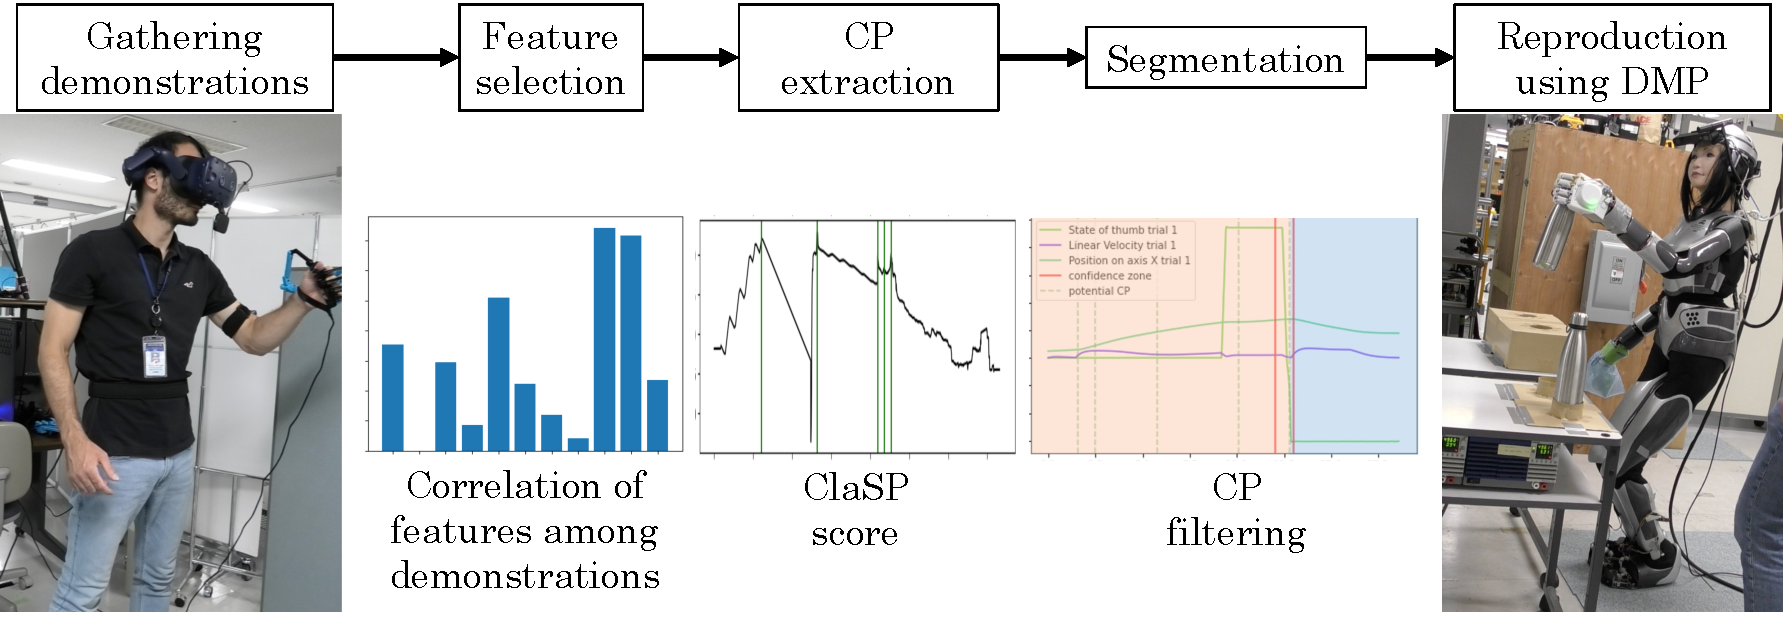
\includegraphics[width=0.85\linewidth]{img/framework.pdf}
  \caption{Proposed task learning and generalization framework. First, we demonstrate the task with a teleoperation device (image on the left). The data is then preprocessed and features that are the most correlated (histogram on the mid-left) are selected for the segmentation with the ClaSP algorithm (image on the middle). This allows for the potential CPs to be identified and filtered with sensor values (image on the mid-right). Finally, we can reproduce the task with Dynamic Movement Primitives on the HRP-4C robot (image on the right).}
  \label{fig:framework}
\end{figure*}

%Our method addresses all the upcited issues in a comprehensive framework (Fig.~\ref{fig:framework}) that combines state-of-the-art LfD techniques with unsupervised automatic segmentation to achieve robust task learning and generalization. We primarily fetch almost all the data available, whether it is kinetic  or sensory, from a small number of demonstrations and automatically selects the most relevant features to study with Dynamic Time Warping (DTW) \cite{dtw} and correlation analysis. Segmentation is achieved with Classification Score Profile (ClaSP) \cite{clasp} and task reproduction and generalization is performed with DMP \cite{ijspeert_movement_2002} \cite{ijspeert_dynamical_2013}. This framework is applied in simulation on the JVRC1 \cite{jvrc} and in real world on the HRP-4C \cite{hrp4} humanoid robot.

\textit{Contributions:} 
The proposed framework integrates state-of-the-art generalization techniques developed mainly for armed robots to complex humanoids, supplemented by a new preprocessing method that automatically selects the most relevant features of the studied task that is then segmented with an adaptation of the ClaSP \cite{clasp} algorithm to multivariate time-series.

\subsection{Outline}

Section \ref{LfD} describes the learning and generalizing framework and the automatic and multisensory segmentation method used in it. Section \ref{results} puts on display the simulation and experimental results. Future work possibilities are finally explored in section \ref{conclusion}.


% \section{Background} \label{Background}

% \subsection{Classification Score Profile}

% The Classification Score Profile is an non-parametric, self-supervised method to segment Time Series (TS). First, the TS is divided into overlapping windows of a fixed length, which is determined using custom statistical analysis algorithm named \textit{Summary  Subsequence Subsequence (SuSS)}. This novel algorithm is one of the features that enables us to use ClaSP even if the TS studied are not periodic. One of the hypothesis that gives high performance segmentation with ClaSP is, indeed, the pseudo-peridiodicity on the Time Series. Yet, even if this hypothesis guarantees good results, there is no theoretical flaw to using ClaSP on generic TS. Other algorithms tested in \cite{clasp} to find the window size, like Fast Fourier Transform, are only efficient in periodic TS, and consequently would not be suitable for our approach.


% Once sequenced into overlapping windows, the TS is hypothetically split at different positions along the TS, creating potential segmentations. For each hypothetical segment, certain characteristics (features) are extracted from all its windows. These features are then used for self-supervision learning.
% More precisely, each hypothetical split is transformed into a binary classification problem. All windows to the left of the split point are assigned the label "$0$," and all windows to the right are labeled "$1$."

% A binary k-Nearest-Neighbor classifier (k-NN) is trained on these features using cross-validation. The cross-validation score of the classifier indicates how dissimilar the windows are on the left side of the hypothetical split from the windows on the right side. By evaluating the self-similarity (intra-segment similarity) of windows on the right side compared to windows on the left side for each offset $i$ along the time series $T$, an point of the TS at index $i$ high score in this context indicates low similarity between the two sides. This self-similarity measure is recorded for each offset i, resulting in what is called the \textit{classification score profile} (simply referred as profile) for the time series T. An example of a ClaSP profile can be seen on Fig.~\ref{fig:ClaSProfile}.

% \begin{figure}[ht]
%   \centering
%   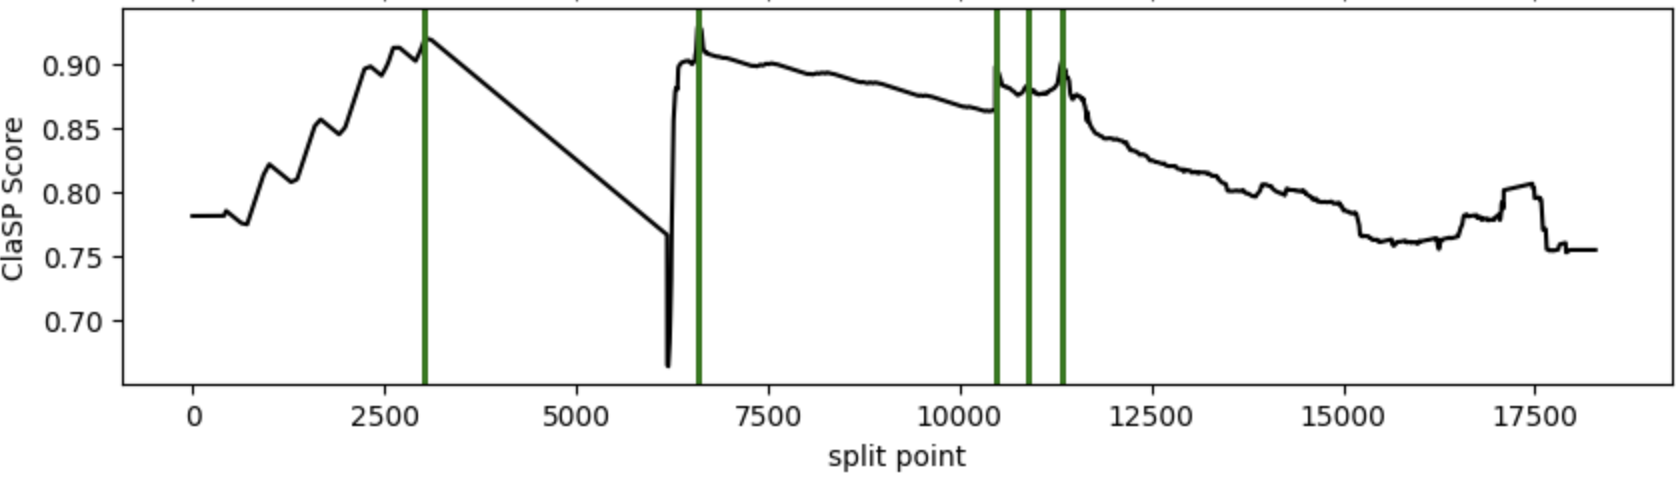
\includegraphics[width=0.45\textwidth]{img/ClaspProfile.png}
%   \caption{Example of ClaSP profile. Some local maxima are selected with the Wilcoxon test to be potential changepoints of the studied time series. The red vertical lines identify the peaks considered as potential changepoints of the considered time series.}
%   \label{fig:ClaSProfile}
% \end{figure}

% To identify potential change points, the ClaSP method looks for local maxima in the classification score profile. By locating these local maxima in the classification score profile, ClaSP highlights regions with significant dissimilarity, thus suggesting candidate positions for segmentation. 

% To this point, ClaSP only detects one CP when taking the global maximum of the score profile. Achieving complete segmentation is done with a recursive algortihm which computes the score profile for the left and right segments, where each local maximum is validated as a true CP only if it statistically significant enough, namely if it passes the non-parametric Wilcoxon rank-sum test. We adapt the segmentation algorithm presented in \cite{clasp} to segment mutltivariate TS, as we expect that a complex task can generally not be fully understood when studying only one feature (position, orientation, sensor value), as relevant as it may be. Our method uses the classes available in the ClaSP code available here (lien github bas de page), but combines the profile computed for different features into one profile that contains underlying information about multiple features. As described in \ref{method_segmentation}, the combination methods explored are averaging the profiles, multiplying all the profiles and also repeating these simple methods but weighting each term by its correlation score as explained in \ref{feature_selection}. The pseudo-code of the algorithm is provided Algorithm \ref{alg:CPD}.


% \begin{algorithm}
%  \caption{Multivariate changepoint detection}
% \begin{algorithmic}[1]
%     \STATE \textbf{Procedure} check\_valid\_cp($profile$, $pq$)
%     \STATE $(\text{cp\_index}, \text{cp\_val}) \leftarrow (\text{argmax(profile)}, \text{max(profile)})$
%     \IF {\text{Wilcoxon\_test}(\text{cpt\_val}) passed}
%         \STATE $pq$.insert(\text{cpt\_val}, (\text{cpt\_idx}, $T$))
%     \ENDIF
%     \STATE \textbf{end procedure}
%     \STATE
%     \STATE \textbf{Procedure} segmentation($T$, $combine\_method$, $min\_segmentSize$)
%     \STATE cpts $\leftarrow$ initialize list
%     \STATE $pq$ $\leftarrow$ initialize max priority queue
%     \STATE profile $\leftarrow$ combine\_method(list\_TS, combine\_method)
%     \WHILE{!$pq$.empty()}
%         \STATE $(\text{cp\_index}, \text{list\_TS}) \leftarrow pq$.get\_maxPriorityValue()
%         \STATE list\_T\_left, list\_T\_right $\leftarrow$ slice\_TS(list\_TS, cp\_index)
%         \IF{length(list\_T\_right) $>$ min\_segmentSize}
%             \STATE right\_profile $\leftarrow$ combine\_method(list\_T\_right, combine\_method)
%             \STATE check\_valid\_cp(right\_profile, pq)
%         \ENDIF
%         \IF{length(list\_T\_left) $>$ min\_segmentSize}
%             \STATE left\_profile $\leftarrow$ combine\_method(list\_T\_left, combine\_method)
%             \STATE check\_valid\_cp(left\_profile, pq)
%         \ENDIF
%         \STATE
%     \ENDWHILE
%     \STATE \textbf{return} cpts
%     \STATE \textbf{end procedure}
% \end{algorithmic}
%  \label{alg:CPD}
% \end{algorithm}

\section{Learning from demonstrations}\label{LfD}

\subsection{Gathering demonstrations}


Building a dataset that covers a wide range of configurations is essential to reach an efficient generalization of the task. To do so, we demonstrated the same task in a similar environment (in the same room, with similar objects on the table, ...) but with different conditions. These include different position parameters (poses of the objects, goal poses, grasping poses) as well as dynamic variables (speed of the movement). Having such a set of demonstrations limits the \textit{covariate  shift}, that's to say the difference of distribution between the training dataset and the real-world cases. Nonetheless, we can not get rid of it in the extent that the action space of a given task in the real world is most often far bigger than what can represent a few demonstrations. In addition to that, our approach is to have a dataset corresponding to what might come natural to a non-professional user.

\subsection{Feature Selection} \label{feature_selection}

Once the demonstrations gathered, the choice of the features to study is another step that often requires the experience of a skilled user. Whereas a majority of LfD techniques selects manually the relevant features to study, we chose to take the measurements of all the sensors available as well as the proprioceptive information, namely 6D Cartesian pose and angular and linear velocites obtained from the robot's solver. Mainly two reasons justify that:

 \begin{itemize}
     \item A non-skilled user has to be able to demonstrate a new task by achieving it in a  natural way wearing the teleoperation device
     \item Capitalize on our similarity with humanoid robots, as recording sensory parameters amounts to add a kind of \textit{sensory integration} in the robot. \textit{Sensory integration} was theorized by Dr A. Jeans Ayres in the field of neuroscience \cite{ayres_improving_1972}. It states that when thinking about achieving some known task, our brain processes not only how to reach the goal (the different steps), but also the sensations we had when achieving this task in the past. 
%This idea was first exploited by P. Pastor et al. in \cite{sensory_skill}. 
A telling example of \textit{sensory integration} is that when we grab an object, the brain area corresponding to our sense of touch activates, and we expect to have some sensation when grabbing an object. 
%In \cite{sensory_skill}, a robot arm corrects his trajectory during grabbing by adding a term that corresponds to his expected force feedback on the gripper.
Thus, taking sensor into account while building the dataset can help to detect phases of the movement \cite{sensory_seg} and to the movement online (after the learning phase). \newline

\end{itemize}


Having gathered a set of demonstrations containing numerous features, we now want to automatically extract the most relevant features to segment the studied task.

A first step is to temporally align the signals in order to compare the features across the dataset. Indeed, our goal is to find the most correlated features. Intuitively, if one feature has the same shape in all the trials, it is likely that it plays a role in defining the task, and will be useful for segmentation, and . In a grasping task, the state of the gripper identifies the different phases of the movement and has the same shape across all the trials.

To align the signals, we use Dynamical Time Warping (DTW). The main idea behind DTW is to find the optimal alignment between the two sequences by warping their time axes. This warping process allows for the matching of similar patterns, despite variations in timing and duration. It works by finding the minimum distance path through a grid or matrix that represents the pairwise distances between elements of the two sequences. \newline


We can then compute a \textit{correlation matrix} for each feature across all trials (Fig.~\ref{fig:corrMat}). The mean of the coefficients of these matrices can therefore be interpreted as the similarity across the datasets. Yet, his first result includes a bias due to the temporal alignment of the signals. Indeed, it is possible to have a dissimilar feature that ends up highly correlated when the signals are aligned. In fact, the distance computed with DTW can be used as a tool to measure similarity. Taking the statistical mean of the pairwise distances for every feature and normalizing the values between 0 and 1, we can penalize the correlation coefficients computed afterwards. We employ the normalized DTW distances as weights for the correlation coefficients, eventually leading to a more objective measure of the relevance of the features. We see in Fig.~\ref{fig:histcorr} that the most correlated features are more detached from the other features.  

\begin{figure}[t]
  \centering
  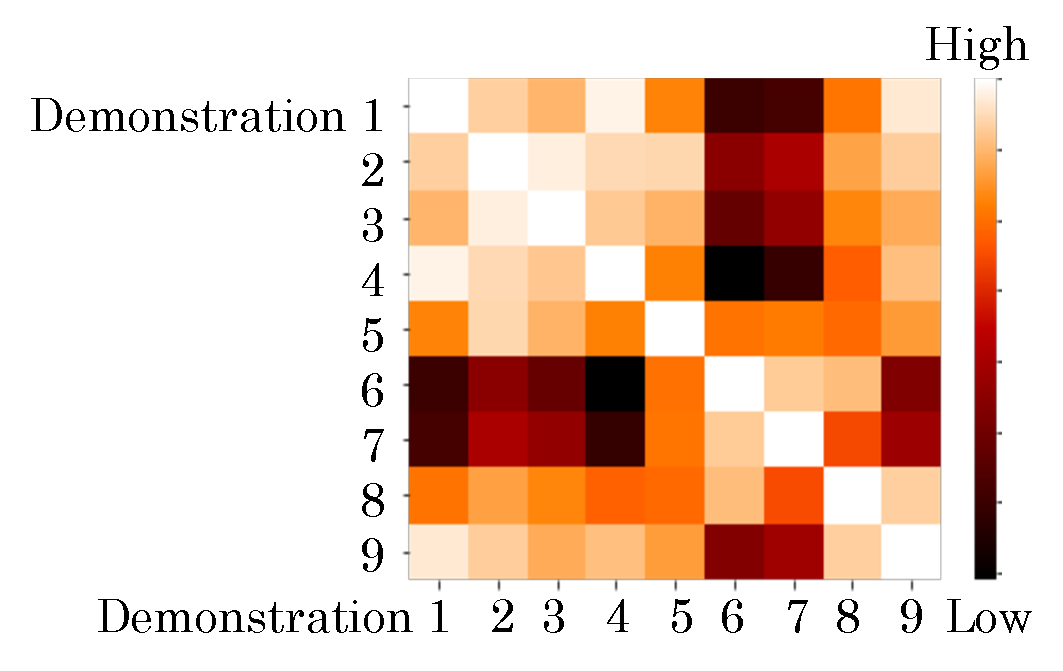
\includegraphics[width=0.4\textwidth]{img/resolCorrMap.pdf}
  \caption{Example of a correlation matrix that shows how one feature (here, the angular velocity of the end-effector) is correlated across the 9 demonstrations.}
  \label{fig:corrMat}
\end{figure}

Finally, we select the features to pass in argument for the segmentation phase. There is a trade-off between selecting the most correlated feature and discarding others - thus possibly missing important information - and choosing too much signals, - thus thwarting the segmentation with uncorrelated features -. In  addition to the most correlated feature $F$, we select the features that are above $CorrCoef_{F} \times T$, with $T$ a threshold that we empirically set at $0.9$, but that could be learned on a dataset containing a sufficient number of tasks. \newline

\begin{figure}[t]
  \centering

  \begin{minipage}[t]{0.49\linewidth}
    \centering
    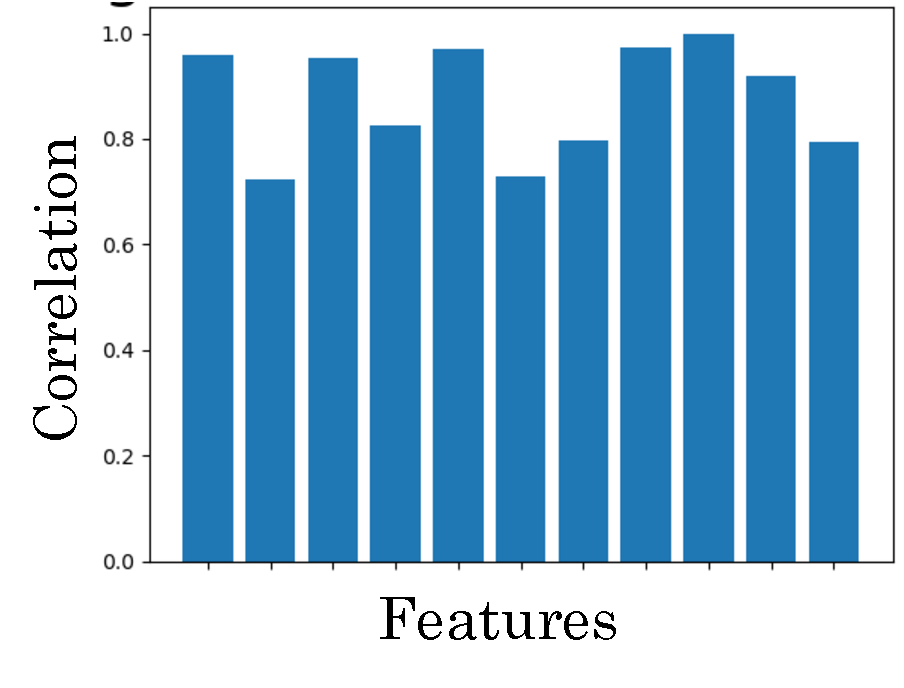
\includegraphics[width=0.95\linewidth]{img/hist_raw.pdf}
    \caption*{(a) Average on the correlation coefficients only}
  \end{minipage}
  \hfill
  \begin{minipage}[t]{0.49\linewidth}
    \centering
    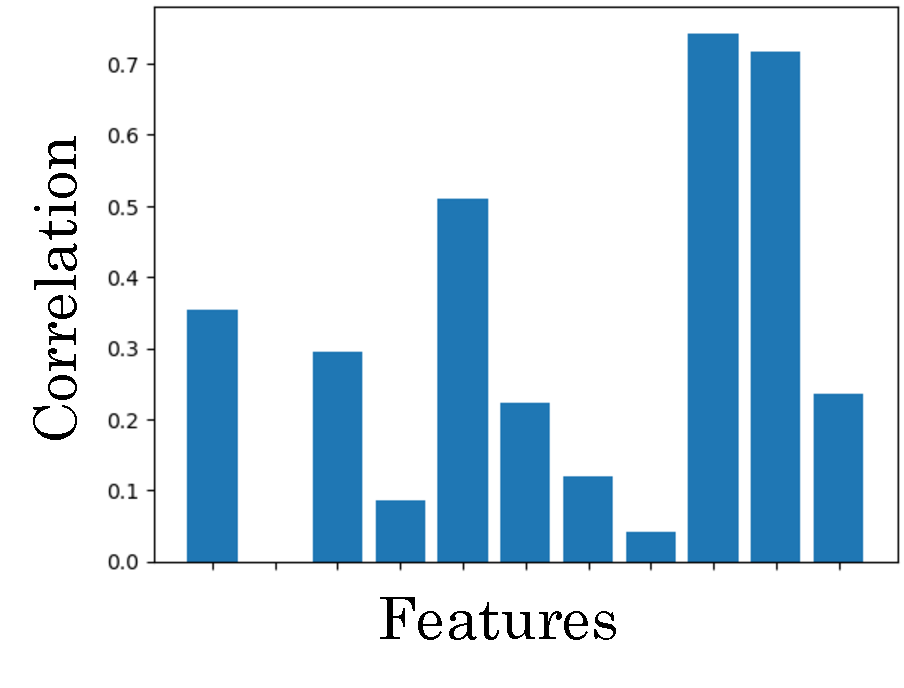
\includegraphics[width=0.95\linewidth]{img/hist_dtw.pdf}
    \caption*{(b) Taking into account the  distance computed with Dynamical Time Warping}
  \end{minipage}

\caption{Histogram of feature correlation across trials. The relevance of the feature is a lot clearer on the right figure that takes into account the distance computed with DTW.}
  \label{fig:histcorr}
\end{figure}

%\textbf{Note:} This correlation analysis is only relevant for demonstrations that are long enough (more than a few seconds). Otherwise, the p-value of the Pearson coefficient \cite{pearson} is above 0.05 and the correlation is very likely to be irrelevant.

\subsection{Segmentation} \label{method_segmentation}

To segment demonstrations, we modified the ClaSP algorithm - originally made for univariate time series - so that we can combine mutliple signals.
%The default parameters of  ClaSP are used, namely the  number of estimators, the number $k$ of neighbours in the $kNN$ algorithm, the window size selection with the  SuSS algorithm. 
%\textcolor{red}{We set the parameter $min\_segmentSize = 500$, so that we only have segmented skills that have a minimum duration of one second (this paremeter excludes CPs $500$ timesteps at the right and left of the considered CP). Indeed, the timestep in mc-rtc and mc-mujoco \cite{singh2023mc} is $0.001s$, so that 1000 timesteps represent segments of 1 second. }

Then, we tried different methods to combine the profiles of the features studied. We considered averaging the profiles and multiply the profiles, but also weighted average and product. Intuitively, the most correlated features have a score profile that is more relevant for the segmentation. Thus, we weight the score profiles with the correlation coefficients computed in \ref{feature_selection} before averaging or multiplying them. As we want to reduce the number of segments, we penalize the score of the points next to potential breakpoints. By computing these CPs recursively, two detected CPs at step $i$ or lower are the bounds of the new time series studied at step $i+1$. Penalization is done with a Kaiser filter on the studied portion of profile (Fig.~\ref{fig:Kaiser}).

\begin{figure}[t]
  \centering
  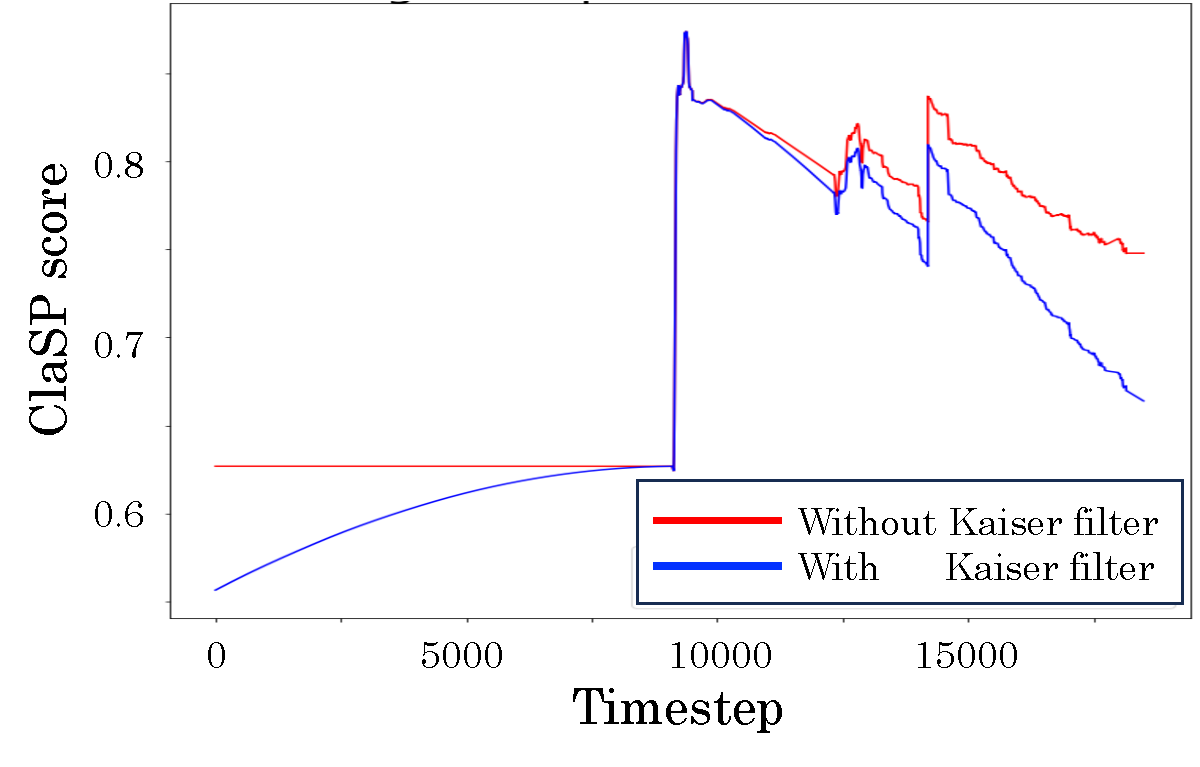
\includegraphics[width=0.4\textwidth]{img/resolKaiser.pdf}
  \caption{ClaSP profile after being filtered with the Kaiser filter. The value of the filtered profile fades on the edges of the profile, thus limiting the possibility to have a big sequence of short subtasks.}
  \label{fig:Kaiser}
\end{figure}

This provides us with a profile that contains potential CPs. We then either discard or validate the CPs with sensory events. Indeed, as explored in \cite{sensory_seg}, new phases in manipulation tasks coincide with sensory events. We reuse this idea and compute a confidence zone around the beginning and ending of sensory events. After having removed the first difference, we detect the sensory events when the data goes from a low state to a high  state and vice-versa, with a threshold set as $0.4\times max\_value$, that empirically gave the best results. Having detected this set of points $S$ for the time series $T$ and the minimum length of a segment $min_s$, we thus obtain the confidence zone:

\begin{equation}
        \bigcup_{s \in S} \left[ \max(0, s - min_s/2),\min(s + min_s/2, \text{len}(T)) \right]
\end{equation}

We finally validate the CPs computed with ClaSP if it belongs to the confidence zone. That way, we have the CPs that corresponds to the sensory events , but we do not accept CPs only if the sensors are activated.

\section{Results and discussion} \label{results}

 We first design a controller to build a dataset in simulation on the JVRC1 robot. To that end, we designed a finite state machine (FSM) controller with mc-rtc\footnote{https://jrl-umi3218.github.io/mc\_rtc/index.html} and mc-mujoco\cite{singh2023mc} to simulate a one-handed grasping task of a stick in 9 different configurations as seen on Fig.~\ref{fig:simSetup}. Having our approach validated with the JVRC-1 robot is essential as it is a simple robot that has only basic capacities , so if our method works on JVRC-1, we can refine it to make it work in real environments. To build a real-world dataset, with the teleoperation device with the HRP-4C robot (Fig.~\ref{fig:setup}). The user has a the visual input of the humanoid's camera, and achieves the task naturally, except that there is no force  feedback on the fingers, meaning that the demonstrator is not constrained by the physical shape of the object during the demonstrations.

\begin{figure}[t]
  \centering
  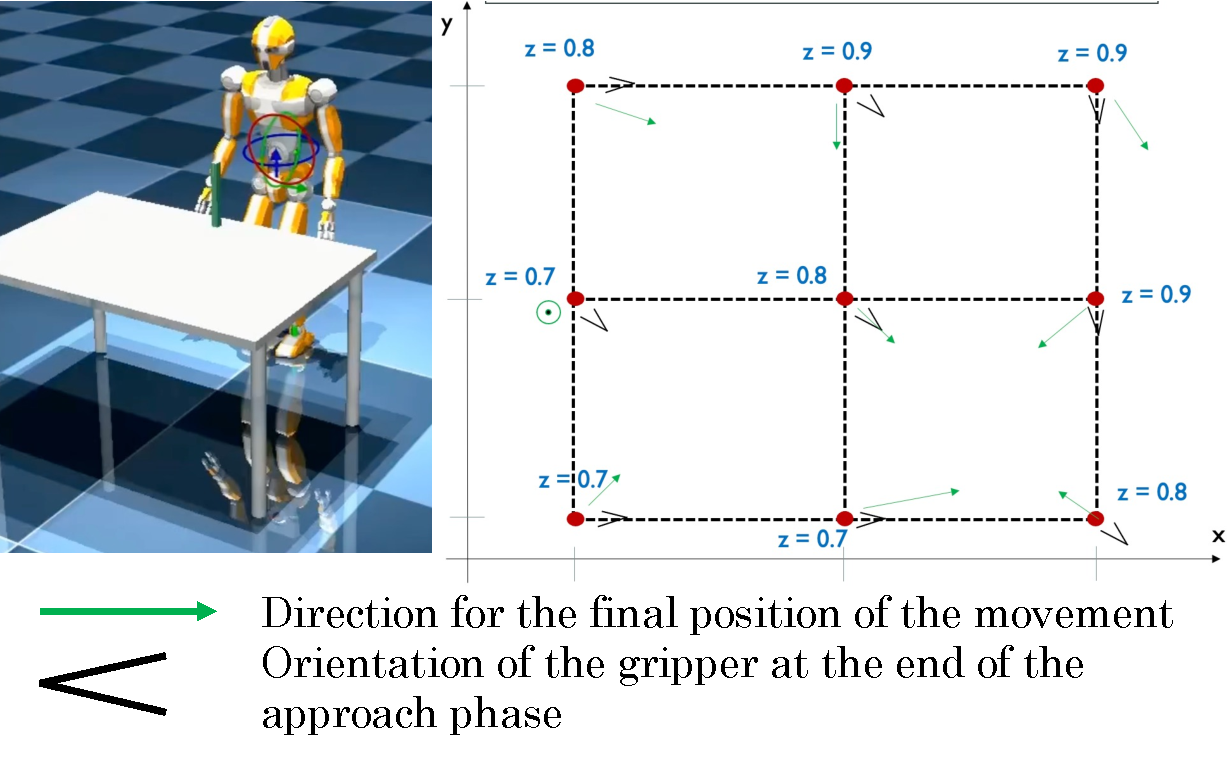
\includegraphics[width=0.49\textwidth]{img/simSetup6.pdf}
  \caption{Setup for the dataset built in simulation. On the left, the Mujoco interface with the JVRC1 \cite{jvrc} at the beginning of the grasping task. On the left, the positions in which is positioned the object to grab, with the pose of the gripper before grasping the stick and the direction in which the latter is lifted.}
  \label{fig:simSetup}
\end{figure}

 The same process is employed to build two datasets for a pushing task, where the goal is merely to push a box on a table. The video of the demonstration with teleoperation are available \href{https://github.com/VictorBbt/Article_TaskGeneralization}{here}.

 In both cases, mc-rtc logs the sensor and proprioceptive values that are used to learn the task. The task can be represented by all its normalized feature values in skill maps as in Fig.~\ref{fig:skillmap}. We then extract appropriate features and segment it into interpretable phases. The features selected for the grasping task were the state of the gripper, the linear velocity and the position on the x axis. The two most important features are the state of the gripper and the linear velocity, which come as no surprise as their profile is not influenced by the start and end position nor by the position of the object. Th movement along the X-axis, on the contrary, seems to be extrinsic to the grasping task, and its influence needs to be investigated, as it is likely to be caused by the dataset. 
 %Nonetheless, the demonstrations provided with the teleoperation device are more similar to each other rather than the dataset built in simulation. \textcolor{red}{That is due to the mechanical constraints of the real-robot. Those are a lot more complex in reality than in simulation.}

 \begin{figure}[t]
  \centering
  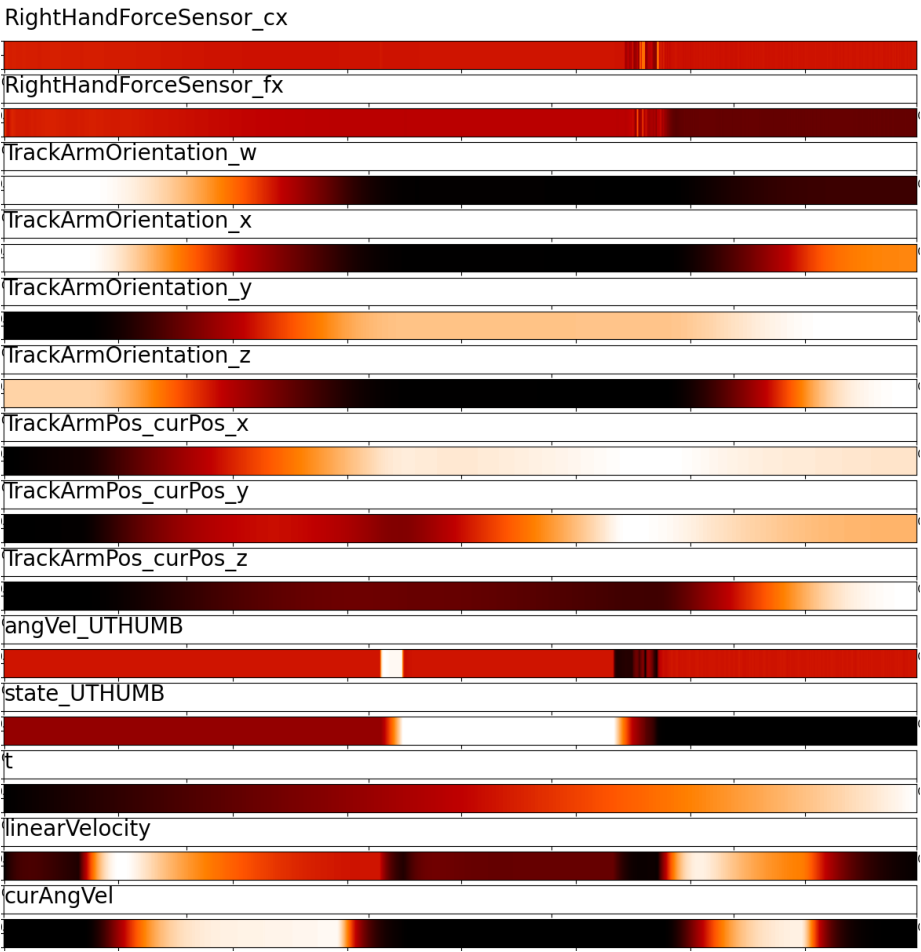
\includegraphics[width=0.45\textwidth]{img/skillMap.pdf}
  \caption{Representation of a grasping task in a skill map. All the features are normalized between 0 and 1. Throughout the entire task (represented in timesteps on the abscissa), we observe the evolution of all the features studied. The higher the value of the normalized feature, the clearer on the skill map. The sensor values on the first two lines show some noise and some discontinuities during the "move object" phase and are used only to compute the confidence zones that will validate the CPs computed with the rest of the features.}
  \label{fig:skillmap}
\end{figure}

To consider that a segmentation is correct, a demonstration of a grasping task must have one CP at the transition between the approach phase (when getting closer to the object) and the moving-object phase (grabbing the object and move it towards an other position). 
%In this work, the object is not released by the robot, the task stops when the robot has lifted the object to a final position. 
Figure~\ref{fig:coloredseg} is a correct segmentation for a grasping task. As we can see, for the considered trial, five potential CPs were identified, but only one is within the confidence zone, thus giving in the end a correct segmentation for this task. Over the dataset, we compute the success rate as the number of trials correctly segmented over the total number of trials.

\begin{figure}[t]
  \centering
  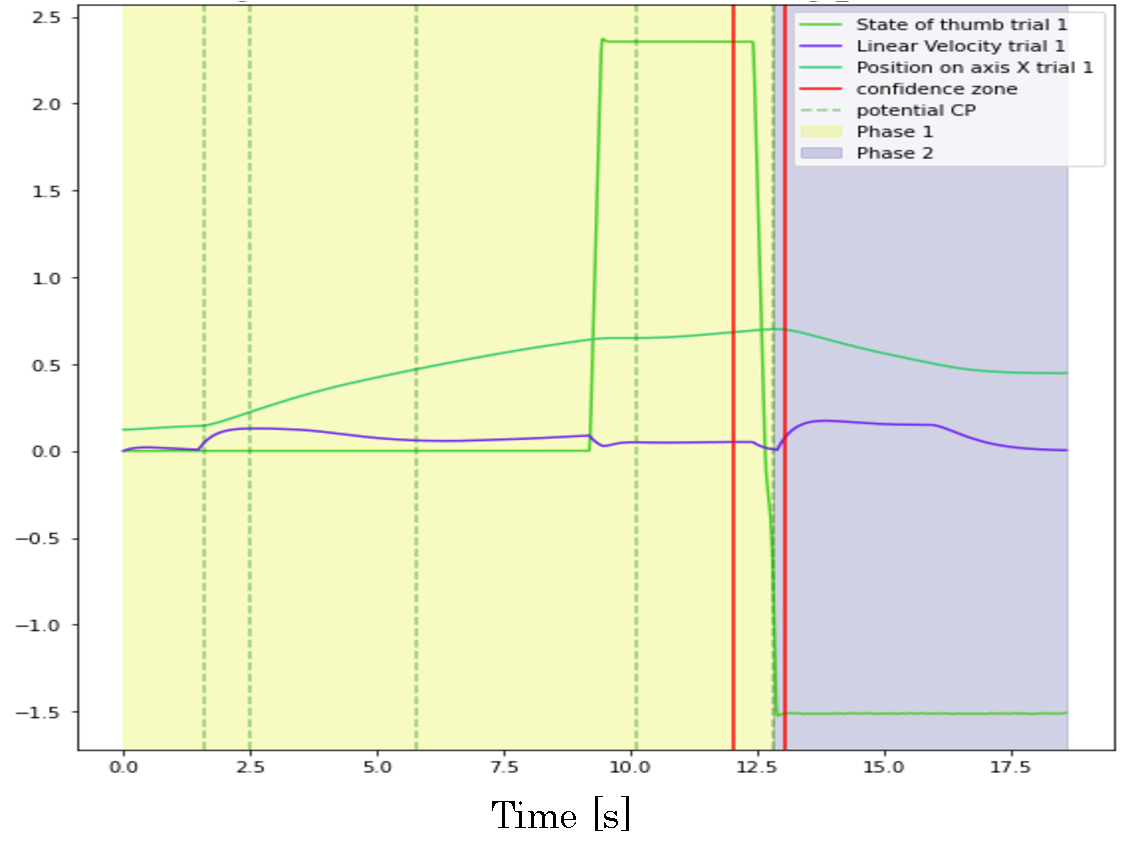
\includegraphics[width=0.5\textwidth]{img/resolSeg.pdf}
  \caption{Correct segmentation of a grasping task. We have one CP inside the confidence zone, that is when the gripper is closing itself on the object. The different phases are coloured in beige (approach phase) and blue (move object phase). As we can see, only one CP is computed in the confidence zone (around 12.5s) bounded by the two red lines.}
  \label{fig:coloredseg}
\end{figure}

As for the pushing task, two CPs are expected to be identified. We have an approach phase when getting closer to the box to push. The pushing phase occurs when the gripper is in contact with the object. Finally, the third phase is simply returning to the initial position.

Note that we consider only correct these segmentations, but even if too much CPs are detected, the movement reproduction with DMPs will still work. In this case, the main issues are that the segments are not interpretable, and that tasks that are not learned in an optimal fashion.


Results are shown on Fig.~\ref{fig:resultsSeg}, and leads us to choose the weighted product method to compute the combined profiles as it shows better performance.
%The first striking point to this study is the lack of efficiency when going sim-to-real. 

While only 50\% of the demonstrations are correctly segmented in the real grasping task, the results obtained in simulation are around 80\%. This is due to noisy logs when using the teleoperation device, especially on sensory data, thus having a confidence zone that is not as accurate as that of the simulated data. We detect too much sensory events, eventually finding too much CPs (suboptimal partition of the task). Teleoperating - and more generally working with - humanoid robots that have complex hybrid behaviors ends up with having noisy data that is harder to exploit than on robots that have less DoFs (robotic arms, quadruped robots, ...). Refining the sensitivity of the sensors could help to address this sim-to-real issue. For instance, learn and classify sensory events, and different characteristics of surfaces (roughness, texture, ...) as it is done in \cite{surface_digital} could help spot the confidence zones, discriminate the nature of the task (e.g, pushing or grasping), eventually computing CPs more accurately.

\begin{figure}[t]
  \centering
  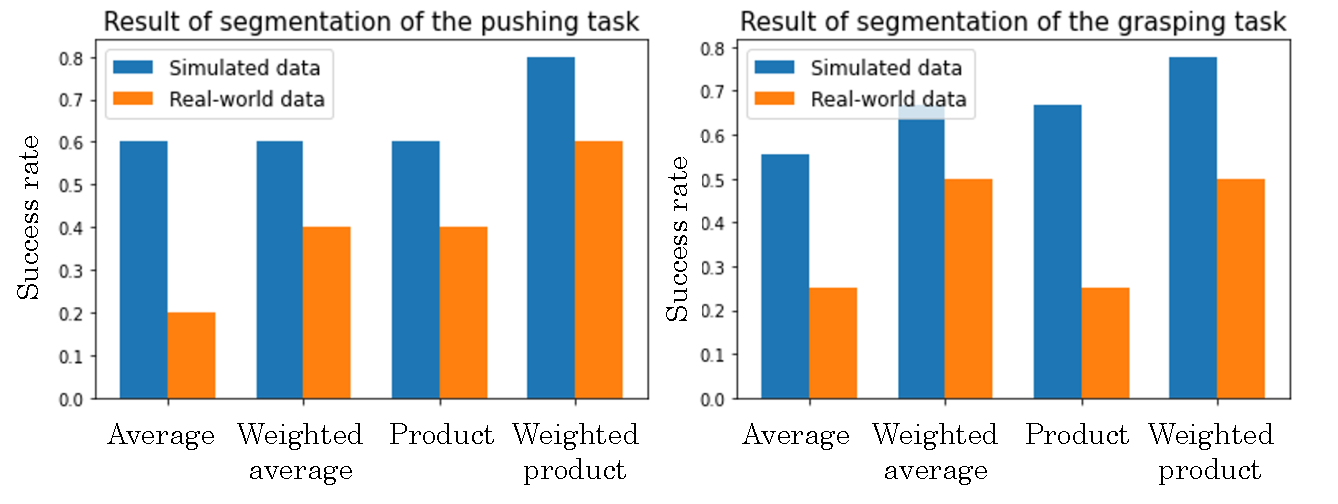
\includegraphics[width=0.5\textwidth]{img/results_segmentation.pdf}
  \caption{Results of the segmentation for the tasks considered. While approximately 80\% of the task are successfully reproduced in simulation (blue), the average percentage is around 50\% on the real robot (orange). These success rates are only on the results of the segmentation of the task, as the reproduction on the real robot is left to future work.}
  \label{fig:resultsSeg}
\end{figure}

Such results can also come from a bigger covariate shift in the real-world dataset. All real-world demonstrations are more similar to each other than that of the simulation dataset. In simulation, the demonstrations by the JVRC1 robot covered a surface of $40 \times 40 cm$ on the table, while it is restrained to $15 \times 15 cm$ on real-world demonstrations by the HRP-4C robot because of the differences in kinematics and dynamics parameters of the robots and controllers. We tend to have correlated features in the real world dataset that should not be correlated for the considered task, eventually leading in computing a profile that have "false" CPs. Those are not discarded because the sensory values are too noisy, thus detecting wrong confidence zones.

To reproduce the task, we compute DMP models for each segment of each demonstration. We learn one DMP for the 6d-pose and one for the state of the gripper. Both are coordinated by the same phase variable.

When performing again this learned skill given a new goal position, we interpolate the new goal with all the precedently learned goals to find a new DMP model that fits to the task. Tasks have been reproduced using this method for the simulated grasping and pushing tasks with 100\% rate of success for the demonstrations that were correctly segmented. Snapshots of the reproduction are showed on Fig.~\ref{fig:reproductionSim}. The execution time to reproduce the task was longer (approximately 1.5 times longer with a processor i9-10885H due to bigger calculations at runtime to run the DMP model). The reproduction on the real robot is a more complex issue that is left to future work, as the main concern is to increase the success rate of segmentation on real-world data beforehand.

\begin{figure}[t]
  \centering
  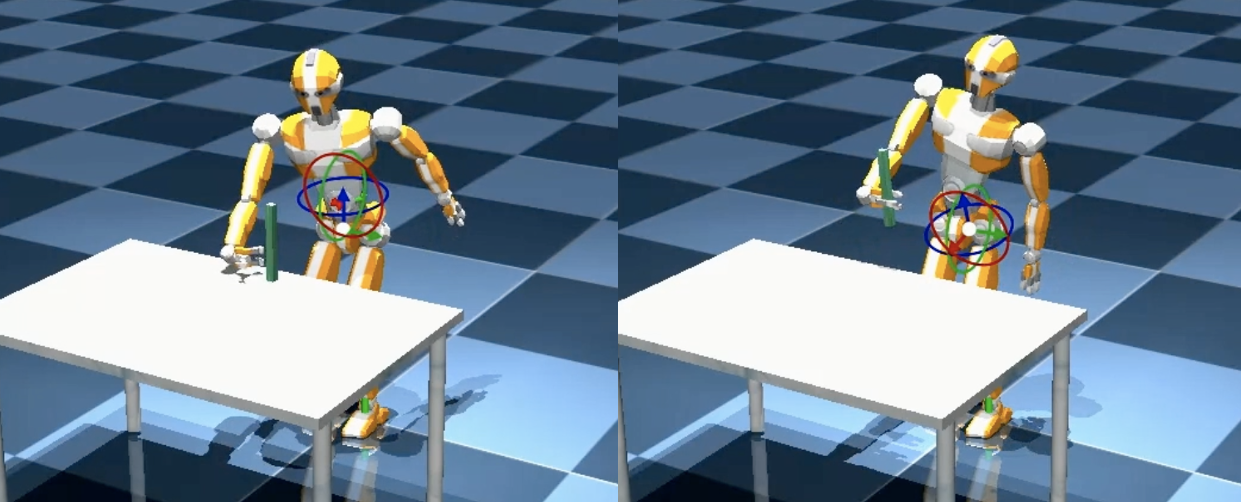
\includegraphics[width=0.45\textwidth]{img/Reproduction.png}
  \caption{Reproduction of the grasping task in simulation on the JVRC1 robot. On the left, the end of the approach phase: the gripper is open near the stick (the position of the stick was manually input). On the right, the end of the lift phase: the robot holds the object in the final position (also manually set).}
  \label{fig:reproductionSim}
\end{figure}

\section{Conclusion and future work}\label{conclusion}

Throughout this work, we presented an end-to-end framework to learn and generalize a new task for humanoid robot by automatically segmenting demonstrations provided in a natural way through teleoperation into reproducible skills. 
%In addition as being a novelty for complex humanoid robots, the proposed approach can be extended to every humanoid robot, and theoretically to every combination of end-effectors (one hand, two hands, legs). 
On top of that, automatically extracting the relevant features with a correlation analysis corroborated with sensory information enables non-skilled users to learn tasks to the robots, therefore fostering humanoids integration in real-world work sites. Our approach, albeit not perfect, shows satisfactory results on simulated data (with around 80\% of success) but has to be refined to be efficient on real-world data. \newline


This work mainly paves the for two potential prolongations.
\begin{itemize}
    \item \textit{Increase the efficiency and the automation.} This would include compute 6d-pose estimation of objects based on visual input, or refine our DMP implementation to make it faster, and add goal-switching and obstacle avoidance as stated in \cite{saveriano_dynamic_2021}. 
    
    \item  \textit{Increase the generalizability and the objectivity.} One could think about replacing the arbitrary thresholds in the feature selection or in the segmentation algorithm by statistical methods, or trying to avoid covariate shift by generating demonstrations through meta-learning \cite{yu_one-shot_2018}.

\end{itemize}
\bibliography{references.bib}
\bibliographystyle{IEEEtran}


\vspace{12pt}

\end{document}

